\documentclass[11pt]{article}

\usepackage{amsmath}
\usepackage{amssymb}
\usepackage{array}
\usepackage{geometry}
\usepackage{enumitem}
\usepackage{float}
\usepackage{cancel}
\usepackage{graphicx}
\usepackage[labelformat=empty]{caption}

\geometry{
	a4paper,
 	left=20mm,
 	top=20mm,
}
 
\setlength{\parindent}{0pt}

\begin{document}

\section{Operators}

\begin{equation*}
\begin{split}
	a | b & :\Leftrightarrow \exists c\ b=ac\ \text{for $a \neq 0$} \\
	a \equiv_m b & :\Leftrightarrow m |(a-b)\ \text{i.e.}\ \exists r\in \mathbb{Z}\ a = b + rm
\end{split}
\end{equation*}

\section{Propositions}

\begin{description}[labelindent=16pt,style=multiline,leftmargin=5.5cm, noitemsep]
	\item[Implication:] $A \rightarrow B :\Leftrightarrow \neg A \lor B $
	\item[Two-sided Implication:] $A \leftrightarrow B :\Leftrightarrow A \equiv B$
	\item[Associativity:] $(F \land G) \land H \equiv F \land (G \land H)$
	\item[Distributive Law:] $(A \land B) \lor C \equiv (A \lor C) \land (B \lor C)$ \filbreak $(A \lor B) \land (C \lor D) \equiv (A \land C) \lor (A \land D) \lor (B \land C) \lor (B \land D)$
	\item[Idempotence:] $F \land F \equiv F$
	\item[Absorption:] $F \land (F \lor G) \equiv F$
	\item[de Morgan's Law:] $\neg (A \land B) \equiv (\neg A \lor \neg B)$ 
\end{description}

\section{Proofs}

To prove a sentence (either true or false) means to show that it's a tautology. The following \textbf{proof patterns} may be used.

\subsubsection{Direct Proof of an Implication}

\paragraph{Example:} $F \rightarrow G$ \\

A \textbf{direct proof of an implication} works by assuming $F$ and then deriving $G$ from $F$.

\begin{equation*}
	F \Rightarrow ... \Rightarrow ... \Rightarrow ... \Rightarrow G
\end{equation*}

\subsubsection{Indirect Proof of an Implication}

\paragraph{Example:} $F \rightarrow G$ \\

An \textbf{indirect proof of an implication} proceeds by assuming $\neg G$ and deriving $\neg F$ under this assumption.

\begin{equation*}
	\neg G \Rightarrow ... \Rightarrow ... \Rightarrow ... \Rightarrow \neg F
\end{equation*}

\subsubsection{Composition of Implications}

\paragraph{Example:} $F \rightarrow G$ and $G \rightarrow H$

\begin{enumerate}
	\item Prove the statement F
	\item Prove the implications $F \Rightarrow G$ and $G \Rightarrow H$
\end{enumerate}

\subsubsection{Case Distinction}

\begin{enumerate}
	\item Define a complete list of cases
	\item Prove the statement for each case separately
\end{enumerate}

\subsubsection{Proof by Contradiction}

Assume that the sentence $F$ is false and derive a false statement from it.

\begin{equation*}
	\neg F \Rightarrow ... \Rightarrow ... \Rightarrow ... \Rightarrow \bot
\end{equation*}

\subsubsection{Existence Proof}

\paragraph{Example:} $\exists x\ P(x)$ \\

Either find a variable which satisfies the sentence (\textbf{constructive}) or proof the existence of such a variable without exhibiting it (\textbf{non-constructive}).

\subsubsection{Proof by Counterexample}

\paragraph{Example:} $\neg\forall x\ P(x)$ \\

Find a variable such that the sentence is wrong.

\subsubsection{Proof by Induction}

\paragraph{Example:} $\forall n\ P(n)$ 

\begin{enumerate}
	\item \textbf{Basis step}: Prove $P(0)$
	\item Assume $P(n)$
	\item \textbf{Induction step}: Prove $P(n + 1)$
\end{enumerate}

\section{Predicate Logic}

\subsection{Rules}

\begin{enumerate}[labelindent=16pt,style=multiline,leftmargin=1.5cm, noitemsep]
	\item $\forall x\ P(x) \land \forall x\ Q(x) \Leftrightarrow \forall x\ (P(x) \land Q(x))$
	\item $\exists x\ (P(x) \land Q(x)) \Rightarrow \exists x\ P(x) \land \exists x\ Q(x)$
	\item $\neg\forall x\ P(x) \Leftrightarrow \exists x\ \neg P(x)$
	\item $\neg\exists x\ P(x) \Leftrightarrow \forall x \ \neg P(x)$
	\item $\exists y \forall x\ P(x, y) \Rightarrow \forall x \exists y\ P(x, y)$
	\item $\forall x\ (\exists x\ P(x) \land P(x)) \lor P(\underline{x})$, where \underline{x} is free
\end{enumerate}

\section{Sets}

\begin{equation*}
\begin{split}
	A \subseteq B & :\Leftrightarrow \forall x\ (x \in A \rightarrow x \in B) \\
	A = B & \Leftrightarrow A \subseteq B \land B \subseteq A \\
	P(A) & := \{S\ |\ S \subseteq A\} \\
	A \cap (B \cup C) & = (A \cap B) \cup (A \cap C) \\
	A \times B & = \{(a, b)\ |\ a \in A \land b \in B\} ,|A\times B| = |A|*|B|\\ 
	\mathcal{P}(\{a,b,c\}) & = \{\emptyset, \{a\}, \{b\}, \{c\}, \{a,b\}, \{a,c\}, \{b,c\}, \{a,b,c\}\} (teilmenge) |\mathcal{P}|=2^{|A|}\\
	 Ordered\_sets & := (a,b):=\{\{a\},\{a,b\}\}
\end{split}
\end{equation*}
A teilmenge of a set is the set itself, every element of the set and the null element.

\section{Relations}

\begin{minipage}[t]{0.5\textwidth}
	\subsection{Reflexive}

	\textbf{Formula:} $a\ \rho\ a$ \\
	\textbf{Set:} $id \subseteq \rho$ \\
	\textbf{Matrix:} Diagonal is all 1\\
	\textbf{Graph:} Every vertex has a loop \\
	\textbf{Examples:} $\leq$, $\geq$, $|$, $\equiv_m$ on $\mathbb{Z}$
	
	\subsection{Transitive}

	\textbf{Formula:} $a\ \rho\ b\ \land\ b\ \rho\ c \Rightarrow a\ \rho\ c$ \\
	\textbf{Set:} $\rho^2 \subseteq \rho$ \\
	\textbf{Examples:} $\leq$, $\geq$, $|$, $<$, $>$, $\equiv_m$ on $\mathbb{Z}$
\end{minipage}
%
\begin{minipage}[t]{0.5\textwidth}
	\subsection{Symmetric}
	
	\textbf{Formula:} $a\ \rho\ b \Leftrightarrow b\ \rho\ a$ \\
	\textbf{Set:} $\rho = \hat{\rho}$\\
	\textbf{Matrix:} Matrix is symmetric \\
	\textbf{Graph:} Undirected graph, possibly with loops \\
	\textbf{Examples:} $\equiv_m$ on $\mathbb{Z}$
	
	\subsection{Antisymmetric}
	
	\textbf{Formula:} $a\ \rho\ b \land b\ \rho\ a \Rightarrow a = b$ \\
	\textbf{Set:} $\rho \cap \hat{\rho} \subseteq id$ \\
	\textbf{Graph:} No cycle of length 2\\
	\textbf{Examples:} $\leq$, $\geq$ on $\mathbb{Z}$ and $|$ on $\mathbb{N}$
\end{minipage}\\

\subsubsection{Relations as Sets}

\begin{description}[labelindent=16pt,style=multiline,leftmargin=4.5cm, noitemsep]
	\item[$a\ \rho\sigma\ b$:] $\exists b\in B: (a\ \rho\ b\ \land\ b\ \sigma\ c)$
	\item[$a\ (\rho\cup\sigma)\ b$:] Either $a\ \rho\ b$ or $a\ \sigma\ b$
	\item[$a\ (\rho\cap\sigma)\ b$:] $a\ \rho\ b$ and $a\ \sigma\ b$
	\item[The empty set $\emptyset$:] symmetric and transitive
\end{description}
\subsubsection{Transitive closure}
\begin{equation}
	p^\star = \cup^\infty_{n=1}p^n
\end{equation}

\subsubsection{Equivalence Relation}
\textbf{Example:} = \\ 
A relation that is reflexive, symmetric, and transitive.\\

The set of elements in $A$ that equivalent to $a \in A$ according to the equivalence relation $\theta$ is called the \textbf{equivalence class} of a.
\begin{equation*}
	[a]_\theta := \{b \in A\ |\ b\ \theta\ a \}
\end{equation*}

The set $A/\theta$ of equivalence classes of $\theta$ on $A$ is a \textbf{partition}. \\
If you are looking for a equivalence relation give the matrix with the above properties.

\emph{Hint:}\\
$a\ \theta\ b \Rightarrow [a] = [b]$\\
$a\ \cancel{\theta}\ b \Rightarrow [a] \cap [b] = \emptyset$

\subsection{Partial Order (Ordnungsrelation)}
\textbf{Example:} $\leq$ and $\geq$ on $\mathbb{Z}, \mathbb{Q}$ or $\mathbb{R}$, $=$ on $\mathbb{N}$\\ 
A relation that is reflexive, antisymmetric, and transitive. \\
If every two elements in a poset are comparable than the Set is \textbf{totally ordered}.\\

Special elements in a poset $(A, \preceq)$ with a subset $S \subseteq A$:

\begin{description}[labelindent=16pt,style=multiline,leftmargin=8cm, noitemsep]
	\item[minimal (maximal) element:] $a \in S$ if there exists no $b \in S$ with $b \prec a$ ($b \succ a$) 
	\item[least (greatest) element:] $a \in S$ if $a \preceq b$ ($a \succeq b$) for all $b \in S$
	\item[lower (upper) bound:] $a \in A$ if $a \preceq b$ ($a \succeq b$) for all $b \in S$
	\item[greatest lower (least upper) bound:] $a \in A$ if a is the greatest (least) element of the set of all lower (upper) bounds of $S$
\end{description}

\begin{figure*}
	\centering
	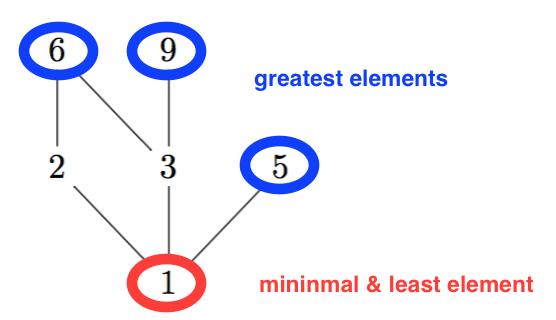
\includegraphics[width=400pt]{images/hasse}
	\caption{Hasse Diagram of the Poset $(\{2,3,4,5,6,7,8,9\};|)$ and $(\{1,2,3,4,6,8,12, 24\};|)$}
\end{figure*}

\subsection{Function}

\begin{description}[labelindent=16pt,style=multiline,leftmargin=3cm, noitemsep]
	\item[injective:] no collisions. $\forall h_1, h_2 \epsilon A$ $h_1 \neq h_2 \Rightarrow f(h_1)\neq f(h_2)$.
	\item[surjective:] every value in the codomain is taken on for some argument
	\item[bijective:] one-to-one mapping (injective and surjective)
\end{description}
\paragraph{ bereinigter pranexform} is when you write a formula with first all the quantifiers and then the formula.

\section{Combinatorics}

\begin{table}[H]
\centering
\begin{tabular}{|p{2cm}|p{6cm}|p{6cm}|}
\hline
                   & \textbf{with repetition} & \textbf{without repetition} \\\hline
\textbf{ordered}   & $n^k$                         							 	  & $\frac{n!}{(n-k)!}$    \\\cline{2-3}
				   & A passcode of length $n$ with $k$ different digits           & How many ways can $k$ places be awarded to $n$ people                       \\\hline
\textbf{unordered} & $\bigl(\begin{smallmatrix}n+k-1\\k \end{smallmatrix} \bigr)$ & $\bigl(\begin{smallmatrix}n\\k \end{smallmatrix} \bigr) = \frac{n!}{k!(n-k)!}$ \\\cline{2-3}
				   & Choose at most $k$ scoops of ice cream from $n$ different flavours   & Select $k$ from $n$ objects                             \\\hline
\end{tabular}
\end{table}

\emph{Hint:} $\bigl(\begin{smallmatrix}n\\0 \end{smallmatrix} \bigr) = \bigl(\begin{smallmatrix}n\\n \end{smallmatrix} \bigr) = 1$, $\bigl(\begin{smallmatrix}n\\1 \end{smallmatrix} \bigr) = \bigl(\begin{smallmatrix}n\\n-1 \end{smallmatrix} \bigr) = n$

\subsection{Countability}

\begin{description}[labelindent=16pt,style=multiline,leftmargin=9cm, noitemsep]
	\item[same cardinality $A \sim B$:] There exists a bijection $A \rightarrow B$
	\item[B has at least the cardinality of A $A \preceq B$:] $A \sim C$ for some subset $C \subseteq B$
	\item[B dominates A $A \prec B$:] $A \preceq B \land A \cancel{\sim} B$
	\item[countable:] $A \preceq \mathbb{N}$
\end{description}

\emph{Hint:} \\
The set $\{0,1\}^* := \{0,1, 00, 01, ...\}$ of \textbf{finite binary sequences} is countable. \\
The set $\{0,1\}^\infty$ is uncountable (Cantor's diagonalization argument). \\
The set \textbf{$A^n$ of $n$-tuples} over A is countable. \\
The \textbf{union of a countable list} of countable sets is countable (can be considered as  tuples).\\
$\mathbb{N}$, $\mathbb{Z}$ und $\mathbb{Q}$ are countable $\mathbb{P}(\mathbb{Z})$ ist uberabzahlbar(=not countable).

\subsection{Inclusion/Exclusion Principle}

\begin{equation*}
	|A \cup B \cup C| = |A| + |B| + |C| - |A\cap B| - |A\cap C| - |B\cap C| + |A\cap B\cap C|
\end{equation*}

\subsection{Double counting principal}
We want to count the subset of A$\times$B(which is a relation). We can a$\epsilon$A the number $m_a$ of b$\epsilon$B such that (a,b)$\epsilon$S. Or the same for B(equal to the sum of ones in the matrix representation).

\subsection{Pigeon hole principal}
If a set of n objects is partitioned into k $<$ n sets, then at least one of these sets contains at least $\frac{n}{k}$ objects

\subsection{Binomial Theorem}

\begin{equation*}
	(x + y)^n = \sum^n_{k=0} \bigl(\begin{smallmatrix}n\\k \end{smallmatrix}\bigr) x^{n-k}y^k
\end{equation*}

\section{Graph Theory}

\subsection{Special Graphs}

\begin{description}[labelindent=16pt,style=multiline,leftmargin=6cm, noitemsep]
	\item[complete graph $K_n$] $n$ vertices, $\frac{n(n-1)}{2}$ edges, $(n)$-regular (every vertex has the same degree n)
.	\item[k regular graph] Each vertex has k neighbours.
	\item[compete bipartite graph $K_{m,n}$] $m+n$ vertices, $mn$ edges, with two vertex subsets $|V_b| = m$ and $|V_w| = n$
	\item[tree:] undirected, connected graph with no cycles and $n-1$ edges.
	\item[hypercube $Q_d$:] \emph{$d$-regular} with $2^d$ vertices and $2^{d-1}d$ edges
	\item[mesh $M_{m,n}$:] $mn$ vertices
\end{description}

\subsection{Traversals}

\begin{description}[labelindent=16pt,style=multiline,leftmargin=4.5cm, noitemsep]
	\item[walk:] sequence of vertices such that consecutive vertices are connected
	\item[tour:] a walk with distinct edges
	\item[circuit:] a tour that ends where it started
	\item[Euler cycle:] a circuit that visits every node exactly once
	\item[Hamiltonian cycle:] a circuit that visits every vertex exactly once
\end{description}

\subsection{Planar Graphs}

For \emph{connected, planar} graphs, the following equations hold:
\begin{description}[labelindent=16pt,style=multiline,leftmargin=4.5cm, noitemsep]
	\item $r  = |E| - |V| + 2$ (number of regions)
	\item $\Sigma_{v \in V}deg(v) = 2|E|$ (sum of the degrees of the regions)
	\item if $|V| \geq 3 \Rightarrow |E| \leq 3|V| - 6$
	\item if $|V| \geq 3$ and bipartite $\Rightarrow |E| \leq 2|V| - 4$
	\item $K_n$ is planar if and only if $n \leq 4$i
\end{description}

Rules to prove \textbf{non-planarity}
\begin{itemize}[noitemsep]
	\item deletion of edges
	\item deletion of singleton vertices
	\item merging neighboring vertices
\end{itemize}

\subsection{Isomorphism}

Two graphs are \textbf{isomorphic} (denoted $\cong$) if there exists a bijection $\pi: V \mapsto V'$ such that 
\begin{equation*}
	\{u,v\} \in E \Leftrightarrow \{\pi(u), \pi(v)\} \in E'
\end{equation*}

\emph{Hint:} Look for cycles with vertices that have a distinct number of degrees. If the graph in question doesn't contain that specific cycle, it can't be isomorph. 
\begin{enumerate}
	\item $|E|+|E^{-}| = 2|E|$ ist gleich der Maximalen Anzahl kanten in Graph.
	\item $\frac{|v|(|v|-1)}{2}$ ist gleich der Maximalen Anzahl kanten in Graph.
\end{enumerate}

\subsection{Trees}
A tree is an undirected connected graph with no cycles. A forest is an undirected graph with no cycles. A leaf is a vertex with degree one. A tree has n-1 edges.

\section{Number Theory}

\subsection{Division}

\emph{Hint:} Every non-zero integer is a divisor of 0. 1 and -1 are divisors of every integer.

\subsection{Greatest Common Divisor}

For integers $a$ and $b$ (not both 0), an integer $d$ is called a $gcd(a,b)$ if $d$ divides both $a$ and $b$ and if every common divisor of $a$ and $b$ divides $d$.

\begin{equation*}
\begin{split}
	d|a\ \text{and}\ d|b\ \text{and}\ c|a \land c|b \Rightarrow c|d \\
	gcd(a,b) :\Leftrightarrow \exists u,v\ ua + vb
\end{split}
\end{equation*}

\subsection{Chinese Remainder Theorem}

\begin{equation*}
\begin{split}
	\text{given}\qquad z & \equiv_{b_1} c_1 \\
	z & \equiv_{b_2} c_2 \\
	z & \equiv_{b_3} c_3 \\
	\text{then}\qquad z & = B_1x_1c_1 + B_2x_2c_2 + B_3x_3c_3 \\
	\text{where}\qquad B_i & = \frac{B}{b_1}\ \text{with}\ B = b_1b_2b_3\ \text{and}\ B_ix_i \equiv_{b_i} 1 \\
	\text{To find different $z$ to satisfy certain constraints}\qquad z' & = z \pm n \cdot B,\ n \in \mathbb{N}
\end{split}
\end{equation*}

\subsection{Extended Euclidean Algorithm}

\begin{equation*}
\begin{split}
	\text{given}\qquad x & = gcd(888, 54) \\
	\text{then}\qquad 888 & = 54(16) + 24 \\
	54 & = 24(2) + \underline{6} \\
	24 & = 6(4) + 0 \\
	\text{to find 6 = u(888) + v(54):}\qquad 6 & = 54 - 24(2) \\
	& = 54 + 24(-2) \\
	& = 54+ (888-54(16))(-2) \\
	& = 54 + (888+54(-16))(-2) \\
	& = 54 + 888(-2) + 54(32) \\
	& = (-2)888 + (33)54
\end{split}
\end{equation*}

\subsection{Ideal}

\begin{equation*}
\begin{split}
	(a,b) & := \{ua + vb | u,v \in \mathbb{Z}\} \\
	(a) & := \{ua | u \in \mathbb{Z}\}
\end{split}
\end{equation*}

For $a,b \in \mathbb{Z}$ there exists $d \in \mathbb{Z}$ such that $(a,b) = (d)$. This is implies that $d$ is the \textbf{gcd} of $a$ and $b$.

\subsection{Least Common Multiple}

$l = lcm(a,b)$ is the common multiple of $a$ and $b$ which divides every common multiple of $a$ and $b$.
\begin{equation*}
	a|l'\ \text{and}\ b|l'\ \Rightarrow l|l'
\end{equation*}

It follows:
\begin{equation*}
	gcd(a,b) \cdot lcm(a,b) = ab
\end{equation*}

\subsection{Modular Arithmetic}

\begin{equation*}
\begin{split}
	R_m(a + b) & = R_m(R_m(a) + R_m(b)) \\
	R_m(ab) & = R_m(R_m(a) \cdot R_m(b)) \\
	R_m(a^{bc}) & = R_m(R_m(a^b)^c)
\end{split}
\end{equation*}

\subsection{Multiplicative Inverses}

The \textbf{congruence equation} has a solution $x \in \mathbb{Z}_m$ if and only if $gcd(a, m) =1$. The solution is unique.
\begin{equation*}
	ax \equiv_m 1
\end{equation*}

The $x$ satisfying the equation is called the \textbf{multiplicative inverse of a modulo m (a Einheit of the Ring)} ($x \equiv_m a^{-1}$ or $x \equiv_m \frac{1}{a}$). 

\subsection{Diffie-Hellmann Key-Agreement Protocol}

The Diffie-Hellmann protocol is based on the \textbf{discrete logarithm problem}. Basically, while $y = R_p(g^x)$ can be computed efficiently, it can't be solved for $x$.

\begin{center}
	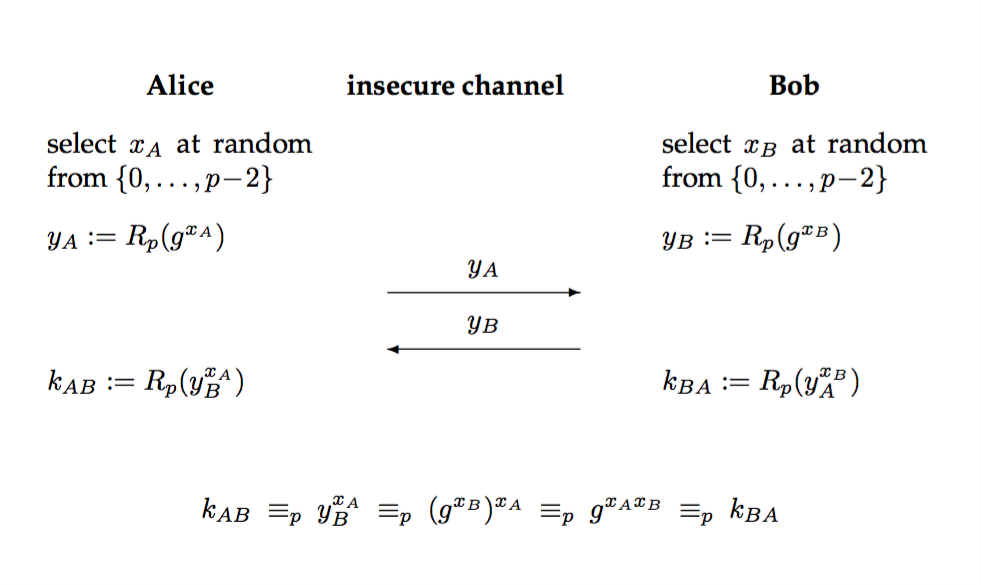
\includegraphics[width=400pt]{images/diffie-hellmann-1}
	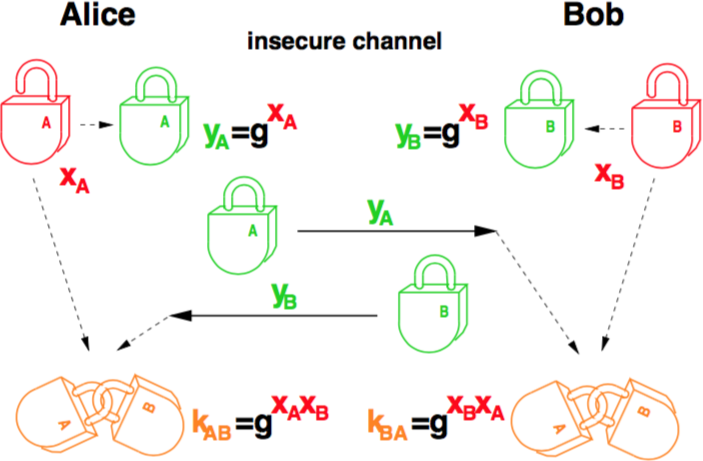
\includegraphics[width=400pt]{images/diffie-hellmann-2}
\end{center}

\subsection{RSA}

A finite group needs $G$ needs to be chosen. Usually, the group $\mathbb{Z}_n^*$ where $n=pq$ is the product of two secret prime numbers. Then $d$ is equal to
\begin{equation*}
	d \equiv_{|G|} e^{-1} \equiv_{(p-1)(q-1)} e^{-1}
\end{equation*}

where $d$ is the \textbf{private key} and the tuple $(n,e)$ is the \textbf{public key}.

\emph{Hint:} It's not possible to calculate $d$ without knowing $G$'s order.

\begin{center}
	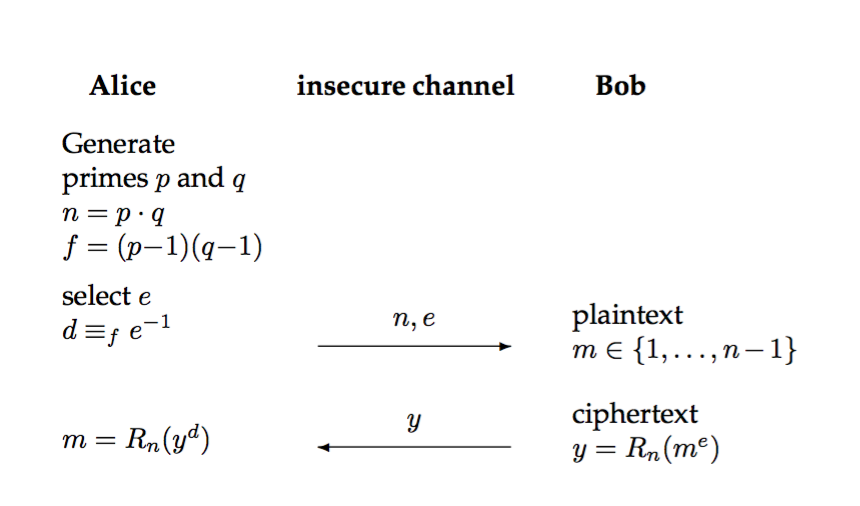
\includegraphics[width=400pt]{images/rsa}
\end{center}

\section{Algebra}

\subsection{Special Properties}

Some special properties of an algebra $\langle S; *, e\rangle$ are

\begin{description}[labelindent=16pt,style=multiline,leftmargin=5.5cm, noitemsep]
	\item[neutral element:] $e \in S$ such that $e * a = a * e = a$
	\item[associativity:] $*$ is associative if $a *(b*c) = (a*b)*c$ for all $a,b,c \in S$ 
	\item[inverse element:] $b$ is the inverse of $a$ if $b * a = a*b = e$
	\item[commutative/abelian:] $a*b = b*a$ for all $a,b \in S$
\end{description}

The \textbf{neutral} and \textbf{inverse element} can have a left and right version. E.g. $e * a = a$ is the left neutral element. However, there is \emph{always only one} neutral/inverse element.

\subsection{Special Algebras}

\begin{table}[H]
\centering
\begin{tabular}{|p{3cm}|p{3cm}|p{6cm}|p{4cm}|}
\hline
                   & \textbf{Notation} 						   & \textbf{Axioms}									& \textbf{Examples} \\ \hline
\textbf{Semigroup} & $\langle S; *\rangle$                     & $*$ is associative 								& \\ \hline
\textbf{Monoid}    & $\langle M; *, e\rangle$                  & $*$ is associative                 				& \\ \cline{3-3}
			       & 										   & $e$ is the neutral element         				& \\ \hline
\textbf{Group}     & $\langle G; *, \hat{}, e\rangle$		   & $*$ is associative                 				& $\langle \mathbb{Z}; +, -,0\rangle$, $\langle \mathbb{Q}-\{0\}; \cdot, ^{-1},1\rangle$, $\langle \mathbb{R}; +, -,0\rangle$ \\ \cline{3-3}
				   &											   & $e$ is the neutral element					    	& \\ \cline{3-3}
				   &											   & every $a \in G$ has an inverse element 			& \\ \hline
\textbf{Ring}      & $\langle R; +, -, 0, \cdot, 1\rangle$	   & $\langle R; +, -, 0\rangle$ is a commutative group & $\mathbb{Z}, \mathbb{Q}, \mathbb{R}, \mathbb{C}$ (commutative) \\ \cline{3-3}
			       &										   & $\langle R; \cdot, 1\rangle$ is a monoid 			& \\ \cline{3-3}
			       &										   & $a(b+c) = ab +ac$ and $(b+c)a = ba + ca$ for all $a,b,c \in R$ & \\ \hline
\textbf{Integral \filbreak Domain (korper)}	&									   & cummutative 						 				& $\mathbb{Z}, \mathbb{Q}, \mathbb{R}, \mathbb{C}$ \\ \cline{3-3}
			       &										   & no zerodividers \filbreak $ab = 0 \Rightarrow a = 0 \lor b = 0$& \\ \hline
\textbf{Field}	   &$GF(p) \equiv \mathbb{Z}_p$& $\langle F - \{0\}; \cdot, ^{-1}, 1\rangle$ is a commutative ring 						 				& $\mathbb{Q}, \mathbb{R}, \mathbb{C}, \mathbb{Z}_p$ \\ \cline{3-3}
			       &										   & every nonzero element is a unit (has an inverse) 	& \\ \hline
\end{tabular}
\end{table}

\emph{Hint:} In order to prove a specific algebra, prove its axioms and that the set is closed in correspondence to its operations, a ring $R^*$ means the ring that only contains units.

\subsection{Groups}

\subsubsection{Direct Product}

The \textbf{direct product of $n$ groups} $\langle G_1; *_1\rangle, ..., \langle G_n; *_n\rangle$ is the group
\begin{equation*}
	\langle G_1 \times ... \times G_n, \star\rangle
\end{equation*}
where the operation $\star$ is component-wise:
\begin{equation*}
	(a_1,..., a_n) \star (b_1,...,b_n) = (a_1 *_1 b_1,...,a_n *_n b_n)
\end{equation*}

\subsubsection{Homomorphism}

A function $\psi$ from a group $\langle G; *, \hat{}, e\rangle$ to a group $\langle H; \star, \hat{}, e'\rangle$ is a group homomorphism if, for all $a$ and $b$
\begin{equation*}
	\psi(a * b) = \psi(a) \star \psi(b)
\end{equation*}

Furthermore, $\psi$ is an \textbf{isomorphism} if it's a bijection.

A group homomorphism satisfies:
\begin{equation*}
\begin{split}
	\psi(e) & = e' \\
	\psi(\hat{a}) & = \widehat{\psi(a)}
\end{split}
\end{equation*}

\subsection{Subgroup}

A subset $H \subseteq G$ of a group $\langle G; *, \hat{}, e\rangle$ is called a subgroup if $\langle H; *, \hat{}, e\rangle$ is \emph{closed} with respect to all operations.

\begin{equation*}
\begin{split}
	& a * b \in H \ \text{for all}\ a,b \in H \\
	& e \in H \\
	& \hat{a} \in H  \ \text{for all}\ a \in H
\end{split}
\end{equation*}

The smallest subgroup of a group $G$ containing the element $g \in G$ is the \textbf{group generated} by $g$:
\begin{equation*}
	\langle g \rangle := \{g^n | n \in \mathbb{Z} \}
\end{equation*}
where the resulting group is called \textbf{cyclic}.\\

\emph{Hint:} The order of a subgroup of a finite group divides its enclosing group's order i.e. $|H|$ divides $|G|$. A subgroup of size two contains e and an element a, a has to be it's own invers: aa=e. A subgroup with a prime order is cyclic and therefore isomorph to $\mathbb{Z}_n,\bigoplus$ and because of $\bigoplus$ is also kommutativ.

\subsubsection{Cyclic Group}

A \textbf{cyclic group} of order $n$ is isomorphic with $\langle \mathbb{Z}_n;\oplus\rangle$. \\

\emph{Hint:} Every group of prime order is cyclic, and in such a group every element except the neutral element is a generator. \\
\emph{Hint:} $\mathbb{Z}_p^*$ is cyclic if and only if $m=2$, $m = 4$, $m = p^e$ or $m = 2p^e$, where p is a prime and $e \geq 1$

\subsubsection{Order}

\paragraph{of a finite group:} $|G|$ is the order of $G$ 
\paragraph{of an element of G:}
The order of $a \in G$ is the least $m \geq 1$ such that $a^m = e$ if such an $m$ exists, and $ord(a) = \infty$ otherwise. \\
\emph{Hint:}  $ord(e) = 1$. If $ord(a) = 2$, then $a^{-1} = a$.

\subsection{Group $\mathbb{Z}_m^*$ and Euler's Function}

$\langle \mathbb{Z}_m^*; \odot, ^{-1}, 1\rangle$ is a group with the set
\begin{equation*}
	\mathbb{Z}_m^* := \{a \in \mathbb{Z}_m\ |\ gcd(a,m) = 1\}
\end{equation*}

The \textbf{Euler function} is defined as follows:
\begin{equation*}
	\varphi(m) = |\mathbb{Z}_m^*| = (p-1)(q-1)\ \text{with}\ n = pq
\end{equation*}
where $p$ and $q$ are prime.

\emph{Hint:} If $p$ is a prime, then $\mathbb{Z}_p^* = \{1,...,p-1\} = \mathbb{Z}_p - \{0\}$
\paragraph{Fermat, euler}
\begin{equation}
	a^{\varphi(m)}\equiv_m 1
\end{equation}
for every prime p and every a not divisible by p
\begin{equation}
	a^{p-1}\equiv_p 1
\end{equation}

\subsection{Polynomials over Fields}

$R[x]$ denotes a \textbf{polynomial ring}, a set of polynomials over $R$.

A polynomial is called \textbf{monic}, if its first coefficient is 1. \\
The polynomial $a(x) \in F[x]$ is called \textbf{irreducible} if it is divisible only by constants and by constant multiples of $a(x)$.
Moreover, $\alpha \in F$ is a \textbf{root} $\Leftrightarrow$ $(x-\alpha)$ divides $a(x)$. \\


\emph{Hint:} Every polynomial of degree $2$ except $x^2 + x + 1$ is reducible. Every irreducible polynomial of degree $\geq 2$  has no roots.

\paragraph{Example:} Polynomial Division on $GF(2)$:

\begin{equation*}
\begin{split}
	& (x^4+x+1) : (x^2+x+1) = x + 2 \\
	&\underline{-(x^3+2x)} \\
	& \quad -2x^2 -2x + 5 \\
	& \quad \underline{-(2x^2 + 4)} \\
	&\qquad -2x +1
\end{split}
\end{equation*}

\paragraph{Example:} Polynomial Interpolation

\begin{equation*}
\begin{split}
	\text{given}\qquad & a(x)\ \text{with}\ a(3) = 2, a(4) = 6, a(5) = 7 \\
	\text{then}\qquad & a(x) = 2\frac{(x-4)(x-5)}{(3-4)(3-5)}+6\frac{(x-3)(x-5)}{(4-3)(4-5)}+7\frac{(x-3)(x-4)}{(5-3)(5-4)} 
\end{split}
\end{equation*}
\subsubsection{Finite fields}
 There exists a finite field with q elements if and only if q is a power of a prime. The prime is called the charakteristik of the field. Moreover, any two finite fields of the same size q are isomorphic.
\subsection{Error-Correcting Codes}

A \textbf{(k,n)-error-correcting code $\mathcal{C}$} over the alphabet $\mathcal{A}$ with $|\mathcal{A}| = q$ is a subset of cardinality $q^k$ of $\mathcal{A}^n$ i.e. one element is of length $n$, with $q^k$ different elements. \\

\emph{Hint:} Usually, $\mathcal{A} = \{0, 1\}$ with $q = 2$ is being considered \\

The \textbf{Hamming distance} between two codewords is the number of positions at which the two codewords differ.

The \textbf{minimum distance} of an error-correcting code $\mathcal{C}$ is the minimal Hamming distance between any two codewords.

A code $\mathcal{C}$ with minimum distance $d$ can correct $t$ errors if and only if $d \geq 2t + 1$.

\section{Logic}

\subsection{Proof System}

A \textbf{proof system} is a quadruple $\Pi = (\mathcal{S}, \mathcal{P}, \tau, \phi)$ with the following components:
\begin{description}[labelindent=16pt,style=multiline,leftmargin=5.5cm, noitemsep]
	\item[set of statements $\mathcal{S}$:] every $s \in \mathcal{S}$ is either $true$ or $false$
	\item[set of proofs $\mathcal{P}$:] e.g. strings over some alphabet
	\item[truth function $\tau$:] defines the meaning (\emph{semantics}) of objects in $\mathcal{S}$
	\item[verification function $\phi$:] $\phi(s, p)=1$ means that $p$ is a valid proof for the statement $s$
\end{description}

The proof system $\Pi = (\mathcal{S}, \mathcal{P}, \tau, \phi)$ is
\begin{description}[labelindent=16pt,style=multiline,leftmargin=3cm, noitemsep]
	\item[sound] if no false statement has a proof \\
				 $\phi(s, p) = 1 \Rightarrow \tau(s) = 1$ 
	\item[complete] if every true statement has a proof \\
				 $\tau(s) = 1 \Rightarrow \exists p \in \mathcal(P)\ \phi(s, p)=1$
\end{description}

\subsection{Syntax and Semantics}

\begin{table}[H]
\centering
\begin{tabular}{|p{3cm}|p{6cm}|p{4cm}|}
\hline
                   			& \textbf{Description} 						   				& \textbf{Notation}	\\ \hline
\textbf{Syntax} 			& alphabet of allowed symbols and which strings are valid	&  \\ \hline
\textbf{Interpretation}  	& an assignment to all variable, predicate, function and constant symbols					& $\mathcal{A}(A) = \{0, 1\}$ \\ \hline
\textbf{Semantics}		  	& a function $\sigma$ assigning to each forumla $F$ and each suitable interpretation $\mathcal{A}$ a truth value& $\sigma(F, \mathcal{A}) = \{0, 1\}$, \filbreak $\mathcal{A}(F)$ \\ \hline
\textbf{Model}			  	& an interpretation $\mathcal{A}$ for which $F$ is true 	& $\mathcal{A} \models F$ \\ \hline

\end{tabular}
\end{table}

\emph{Hint:} $F \models G$ means that every model for $F$ is also a model for $G$.

\subsubsection{Structure}

A \textbf{structure} is a tuple $\mathcal{A} = (U, \phi, \psi, \xi)$ with the following components:
\begin{description}[labelindent=16pt,style=multiline,leftmargin=3cm, noitemsep]
	\item[universe $U$:] nonempty set
	\item[function $\phi$:] assigns to each function symbol a function $U^k \mapsto U$
	\item[function $\psi$:] assigns to each predicate symbol a function $U^k \mapsto \{0,1\}$
	\item[function $\xi$:] assigns to each variable symbol a value in $U$
\end{description}

\subsection{Calculi}

A \textbf{derivation rule} is a rule for deriving a formula from a set of formulas. $G$ can be derived from the set $\{F_1,...,F_k\}$ by rule $R$:
\begin{equation*}
	\{F_1,...,F_k\} \vdash_R G
\end{equation*}

A \textbf{calculus} $K$ is a finite set of derivation rules $K = \{R_1,...,R_m\}$. It is
\begin{description}[labelindent=16pt,style=multiline,leftmargin=4cm, noitemsep]
	\item[sound/correct] if and only if every derivation rule is correct
	\item[complete] if $F$ is a logical consequence of $M$, then $F$ can be derived from $M$ using $K$
\end{description}

\subsection{Normal Forms}

\subsubsection{Conjunctive Normal Form (CNF)}
\begin{equation*}
	F = (L_{11} \lor ... \lor L_{1m_1}) \land ... \land (L_{n1} \lor ... \lor L_{nm_n})
\end{equation*}

\subsubsection{Disjunctive Normal Form (DNF)}
\begin{equation*}
	F = (L_{11} \land ... \land L_{1m_1}) \lor ... \lor (L_{n1} \land ... \land L_{nm_n})
\end{equation*}

\emph{Hint:} Every formula is equivalent to a formula in \textbf{CNF} and \textbf{DNF}.

\subsection{Resolution Calculus}

Given a Formula $F$ in $CNF$, one can transform it into a set of clauses:
\begin{equation*}
	\mathcal{K}(F) = \{\{L_{11},...,L_{1m_1}\},...,\{L_{n1},...,L_{nm_1}\}\}
\end{equation*}

A clause $K$ is then a \textbf{resolvent} of clauses $K_1$ and $K_2$ if there is a literal $L$ such that $L \in K_1$ and $\neg L \in K_2$
\begin{equation*}
	K = (K_1 - \{L\}) \cup (K_2 - \{\neg L\})
\end{equation*}

This derivation is denoted as follows:
\begin{equation*}
	\{K_1, K_2\} \vdash_{res} K
\end{equation*}

\emph{Hint:} A set $M$ of formulas is unsatisfiable if and only if $\mathcal{K}(M) \vdash_{res} \emptyset$

\subsubsection{Prenex Form}

In order to bring a formula into prenex form
\begin{enumerate}[labelindent=16pt,style=multiline,leftmargin=1.5cm, noitemsep]
	\item Resolve all name collisions
	\item Pull the quantifiers to the front by inverting them every time they surpass a $\neg$.
\end{enumerate}

\end{document}
